This subsection describes the experiments that uncovers the best combination of hidden layers, neurons and epochs as well as the different strategies. Based on the above analysis of wind production influences the network will be tested with combinations of the following input parameters:

\begin{itemize}
\item Wind speed;
\item Air density;
\item Consumption;
\item Time of day;
\item Temperature;
\item Wind direction;
\item Last known production;
\item Date;
\end{itemize}

Furthermore, experiments are needed to investigate the influence of data manipulation and statistical inputs as presented in Section~\ref{sec:usingStatisticalInput}. 

\todo{DRAWING OF NETWORK}

\subsection{Experiment Series One - Selection of input parameters}
The first experiment series is an attempt to find the best constitution of network input parameters based on the analysis in Section~\ref{sec:windPowerAnalysis}. All test results can be see in Appendix~\ref{sec:windResultsAppendix} and have been carried out naively with only normalization - top 20 will be shown here. Since the co-relation between wind production and wind speed is very significant it will always be included as a core input parameter in all test combinations.

\footnotesize
\begin{center}
\begin{longtable}{|c|c|c|c|c|c|c|c|c|c|}
\hline
\textbf{WS} & \textbf{AD} & \textbf{C} & \textbf{T} & \textbf{WD} & \textbf{L-P} & \textbf{Mo}& \textbf{ToD} & \textbf{MAE} & \textbf{Rank} \\
\hline
\endfirsthead
\multicolumn{9}{c}%
{\tablename\ \thetable\ -- \textit{Continued from previous page}} \\
\hline
\textbf{WS} & \textbf{AD} & \textbf{C} & \textbf{T} & \textbf{WD} & \textbf{L-P} & \textbf{Mo}& \textbf{ToD} & \textbf{MAE} & \textbf{Rank} \\
\hline
\endhead
\hline \multicolumn{9}{r}{\textit{Continued on next page}} \\
\endfoot
\hline
\endlastfoot
\arrayrulecolor{light-gray}
 x &  x &  x &  &  &  x &  &  x & 125.31 \\ \hline
 x &  &  x &  &  &  x &  &  x & 128.35 \\ \hline
 x &  x &  x &  &  &  x &  x &  x & 134.73 \\ \hline
 x &  &  x &  x &  &  x &  &  x & 136.2 \\ \hline
 x &  x &  x &  x &  &  x &  &  x & 139.01 \\ \hline
 x &  &  x &  &  x &  x &  x &  x & 141.94 \\ \hline
 x &  x &  x &  x &  &  x &  x &  x & 142.72 \\ \hline
 x &  x &  x &  &  x &  x &  &  x & 143.51 \\ \hline
 x &  &  x &  &  x &  x &  &  x & 144.39 \\ \hline
 x &  x &  x &  &  x &  &  x &  x & 147.46 \\ \hline
 x &  &  x &  x &  x &  x &  &  x & 148.52 \\ \hline
 x &  x &  x &  x &  x &  x &  &  x & 150.27 \\ \hline
 x &  &  x &  x &  x &  &  &  x & 151.49 \\ \hline
 x &  x &  x &  &  x &  x &  x &  x & 156.04 \\ \hline
 x &  x &  x &  x &  x &  x &  x &  x & 156.39 \\ \hline
 x &  &  x &  x &  &  x &  x &  x & 159.04 \\ \hline
 x &  &  x &  &  &  x &  x &  x & 159.97 \\ \hline
 x &  x &  x &  x &  x &  &  &  x & 162.45 \\ \hline
 x &  x &  x &  x &  x &  &  x &  x & 164.28 \\ \hline
 x &  &  x &  x &  x &  x &  x &  x & 169.88 \\ \hline
 x &  &  x &  x &  x &  &  x &  x & 175.32 \\ \hline
\caption{Wind Production Input Parameter Test Top 10}
\end{longtable}
\label{table:windProdInputParamsTop10}
\end{center}
\normalsize
\todo{see appendix}

The results vary from the best MAE at 116.08 to the worst being 489.6. What is obvious from the table in Appendix~\ref{sec:windResultsAppendix} is that date clearly makes the prediction worse. All results from rank 82-128 have month as an input parameter. The month reflects seasonality. In the other end of the scale it is inclusions of the last known production and time of day matrix that ranks the highest. This correspond well with the analysis in Section~\ref{sec:windPowerAnalysis} where the relationship between production and time of day is clear. The usage of the matrix implementation makes the benefit even better because each of the hours has its own value instead of only one value representing all hours (see Section~\ref{sec:Matrix}). The analysis also established that the wind production does not differ much from one hour to the next as which is reflected in the last known production --- more sophisticated attempts with statistic will be in experiments to come. What can come as a surprise is that consumption is not represented better in the top rankings since of its co-relation to the wind production.
The best ranked combination of parameters will be the basis for all coming experiments. The prediction for 400 hours can be seen in Figure~\ref{fig:bestCombiForecast400Hours}.

\begin{figure}[H]
\centering
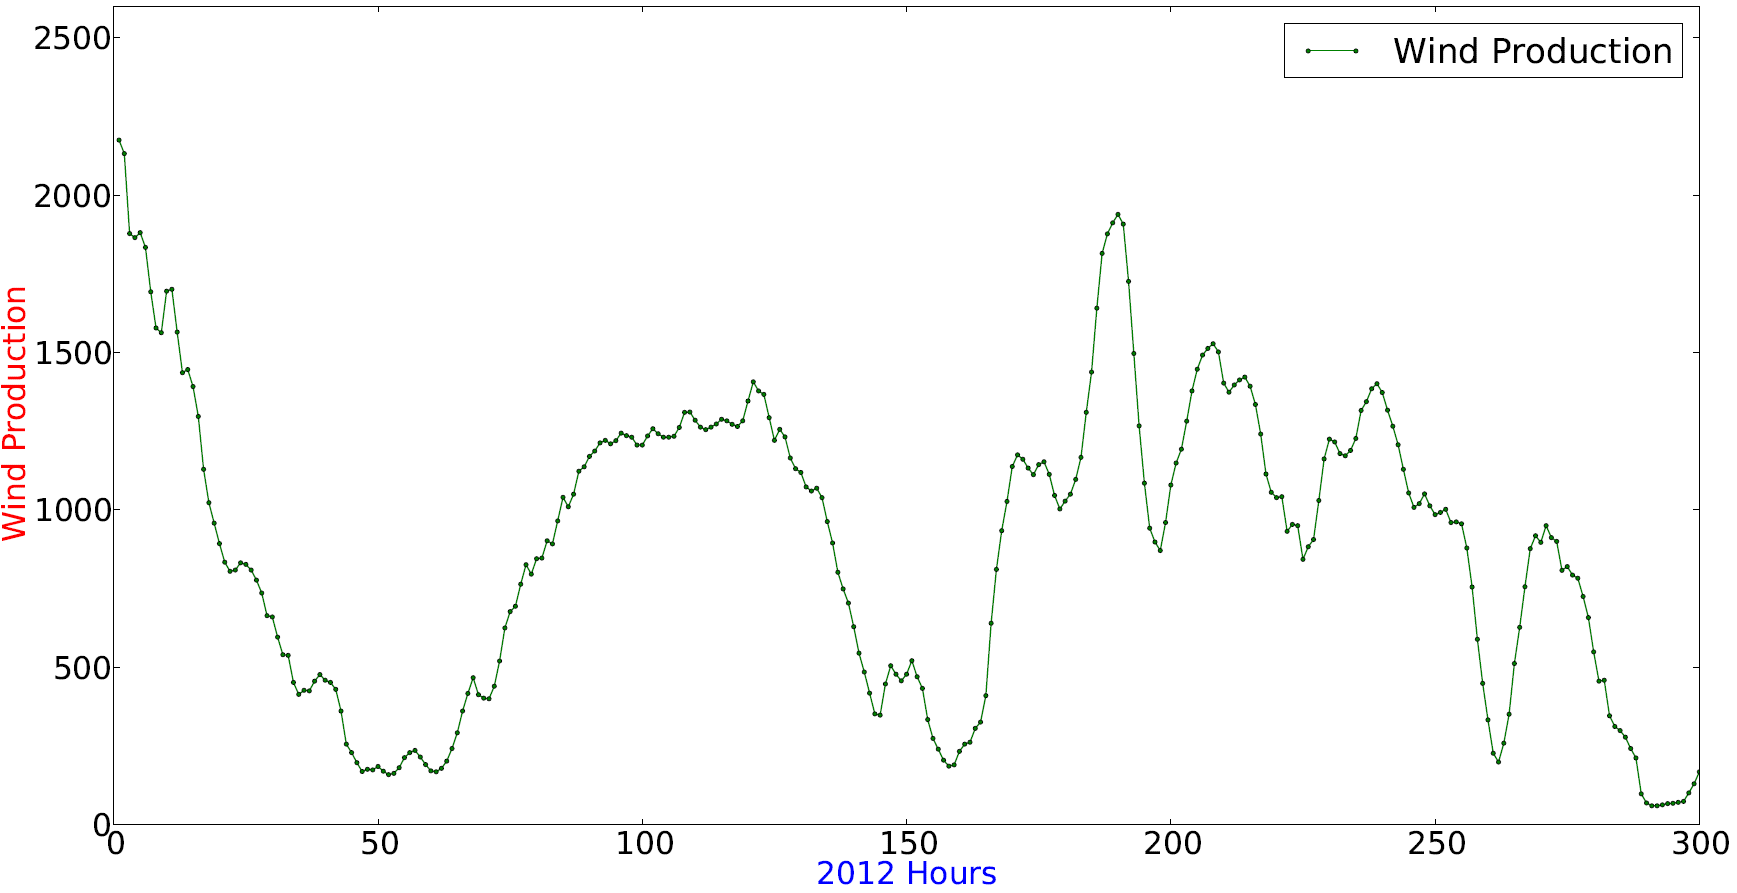
\includegraphics[width=0.99\linewidth,natwidth=898,natheight=587]{billeder/productionTendency400Hours.png}
\caption{Wind production development for 400 hours in 2012}
\label{fig:bestCombiForecast400Hours}
\end{figure}   


The experiments to come will be based on the following input parameters:
\begin{itemize}
\item Wind speed;
\item Air density;
\item Consumption;
\item Temperature;
\item Last known production;
\item Time of day as a matrix;
\end{itemize}

\subsection{Experiment Two - Data Manipulation}
The above inputs with matrix
\footnotesize
\begin{center}
\begin{longtable}{|c|c|c|c|c|c|c|c|c|c|c|}
\hline
\textbf{WS} & \textbf{AD} & \textbf{C} & \textbf{T} & \textbf{WD} & \textbf{L-P} & \textbf{D}& \textbf{ToD} & \textbf{M} & \textbf{MAE} & \textbf{Rank} \\
\hline
\endfirsthead
\multicolumn{10}{c}%
{\tablename\ \thetable\ -- \textit{Continued from previous page}} \\
\hline
\textbf{WS} & \textbf{AD} & \textbf{C} & \textbf{T} & \textbf{WD} & \textbf{L-P} & \textbf{Mo}& \textbf{ToD} & \textbf{Ma} & \textbf{MAE} & \textbf{Rank} \\
\hline
\endhead
\hline \multicolumn{10}{r}{\textit{Continued on next page}} \\
\endfoot
\hline
\endlastfoot
\arrayrulecolor{light-gray}
 x &  x &  x &  x &  &  x &  &  &  x & 116.08 & \#1 \\ \hline
 x &  &  x &  &  &  x &  &  &  x & 118.13 & \#2 \\ \hline
 x &  &  &  &  &  x &  &  &  x & 119.69 & \#3 \\ \hline
 x &  &  x &  x &  x &  x &  &  &  x & 119.81 & \#4 \\ \hline
 x &  x &  x &  x &  x &  x &  &  &  x & 119.88 & \#5 \\ \hline
 x &  x &  &  x &  &  x &  &  &  x & 122.59 & \#6 \\ \hline
 x &  &  &  x &  &  x &  &  &  x & 123.08 & \#7 \\ \hline
 x &  x &  &  &  &  x &  &  &  x & 123.4 & \#8 \\ \hline
 x &  &  x &  &  x &  x &  &  &  x & 123.7 & \#9 \\ \hline
 x &  x &  &  &  x &  x &  &  &  x & 124.42 & \#10 \\ \hline
\caption{Wind Production Input Parameter Test Top 10}
\end{longtable}
\label{table:windProdInputParamsTop10}
\end{center}
\normalsize
\todo{see appendix}

\subsection{Experiment Two - Statistical Inputs}
Statistics. This subsection is experimenting with the concepts described in Section~\ref{sec:usingStatisticalInput}.

\todo{also different size of dataset}

\footnotesize
\begin{center}
\begin{longtable}{|c|c|}
\hline
\textbf{Hours} & \textbf{MAE} \\
\hline
\endfirsthead
\multicolumn{2}{c}%
{\tablename\ \thetable\ -- \textit{Continued from previous page}} \\
\hline
\textbf{Hours} & \textbf{MAE} \\
\hline
\endhead
\hline \multicolumn{2}{r}{\textit{Continued on next page}} \\
\endfoot
\hline
\endlastfoot
\arrayrulecolor{light-gray}
20 & 118,15 \\ \hline
8 & 119,58 \\ \hline
12 & 121,54 \\ \hline
4 & 122,51  \\ \hline
16 & 123,87 \\ \hline
24 & 124,89 \\ \hline
6 & 129,32 \\ \hline
2 & 137,55 \\ \hline
\caption{Prediction With Historical Volatility and different hours}
\end{longtable}
\label{table:historicalVoltalityHours}
\end{center}
\normalsize

\begin{center}
\begin{longtable}{|c|c|}
\hline
\textbf{Hours} & \textbf{MAE} \\
\hline
\endfirsthead
\multicolumn{2}{c}%
{\tablename\ \thetable\ -- \textit{Continued from previous page}} \\
\hline
\textbf{Hours} & \textbf{MAE}\\
\hline
\endhead
\hline \multicolumn{2}{r}{\textit{Continued on next page}} \\
\endfoot
\hline
\endlastfoot
\arrayrulecolor{light-gray}
2 & 114,71 \\ \hline
8 & 116,09 \\ \hline
12 & 117,33\\ \hline
4 & 117,49  \\ \hline
16& 118,09  \\ \hline
20 & 119,35 \\ \hline
6 & 120,64 \\ \hline
24 & 121,67 \\ \hline
\caption{Prediction With Skewness and different hours}
\end{longtable}
\label{table:skewnessHours}
\end{center}
\normalsize


\begin{center}
\begin{longtable}{|c|c|}
\hline
\textbf{Hours} & \textbf{MAE} \\
\hline
\endfirsthead
\multicolumn{2}{c}%
{\tablename\ \thetable\ -- \textit{Continued from previous page}} \\
\hline
\textbf{Hours} & \textbf{MAE} \\
\hline
\endhead
\hline \multicolumn{2}{r}{\textit{Continued on next page}} \\
\endfoot
\hline
\endlastfoot
\arrayrulecolor{light-gray}
24 & 119,73 \\ \hline
12 & 126,62 \\ \hline
20 & 126,84 \\ \hline
16 & 129,87 \\ \hline
6 & 135,56 \\ \hline
4 & 140,18 \\ \hline
8 & 141,36 \\ \hline
2 & 146,13 \\ \hline
\caption{Curve Analysis on different hours}
\end{longtable}
\label{table:curveAnalysisHours}
\end{center}
\normalsize

\begin{center}
\begin{longtable}{|c|c|}
\hline
\textbf{Hours} & \textbf{MAE} \\
\hline
\endfirsthead
\multicolumn{2}{c}%
{\tablename\ \thetable\ -- \textit{Continued from previous page}} \\
\hline
\textbf{Hours} & \textbf{MAE} \\
\hline
\endhead
\hline \multicolumn{2}{r}{\textit{Continued on next page}} \\
\endfoot
\hline
\endlastfoot
\arrayrulecolor{light-gray}
Skewness & 114,71 \\ \hline
Volatility & 118,15 \\ \hline
Scatter & 118,61 \\ \hline
Curve Analysis & 119,73 \\ \hline
\caption{Comparison of the approaches}
\end{longtable}
\label{table:comparisonStatistics}
\end{center}
\normalsize

\todo{say something clever about them}.
Also tried scatter as presented~\cite{singhal2011electricity}. This achieved a MAE of 118.61. A combination of the approaches is illustrated in Table~\ref{table:idealCombination}.

\begin{center}
\begin{longtable}{|c|c|c|}
\hline
\textbf{Hours} & \textbf{MAE} & \textbf{Rank} \\
\hline
\endfirsthead
\multicolumn{3}{c}%
{\tablename\ \thetable\ -- \textit{Continued from previous page}} \\
\hline
\textbf{Hours} & \textbf{MAE} & \textbf{Rank} \\
\hline
\endhead
\hline \multicolumn{3}{r}{\textit{Continued on next page}} \\
\endfoot
\hline
\endlastfoot
\arrayrulecolor{light-gray}
2 & 114.71 & \#1 \\ \hline
\caption{Ideal combination}
\end{longtable}
\label{table:idealCombination}
\end{center}
\normalsize






\todo{better with or without trimming?}


\todo{do 1-12-24 step ahead to show the "carry-with"-error} 


\subsection{Experiment Three - Prediction Strategies}

\subsection{Experiment Four - Black Box Optimization}
Statistics


\subsection{Experiment Five - Performance Optimization}
The impact of different Layers/Neurons/Epochs combinations is huge and the results is shown here.

\begin{table}[H]
\centering  % used for centering table
\begin{tabular}{c c c c c} % centered columns (3 columns)
ANN Type & Epochs & MAE & MPE & Rank \\ [0.5ex] % inserts table 
%heading
\hline                  % inserts single horizontal line
ANN & 500 & 0 & 0 & 0 \\ % inserting body of the table
ANN & 1000 & 0 & 0 & 0 \\
ANN & 2000 & 0 & 0 & 0 \\
ANN & 2500 & 0 & 0 & 0 \\ [1ex] % [1ex] adds vertical space
\hline %inserts single line
\end{tabular}
\caption{Table showing the performance of different data manipulation approaches.} % title of Table
\label{table:performanceOpti} % is used to refer this table in the text
\end{table} 
